\documentclass[tikz]{standalone}
\usepackage{tikz}

\definecolor{codeblue}{RGB}{69, 161, 248}
\definecolor{codegray}{RGB}{40, 40, 40}
\usetikzlibrary{shapes,arrows}
\tikzstyle{decision} = [diamond, draw, fill=codegray, text=white,
    text width=4.5em, text badly centered, node distance=3cm, inner sep=0pt]
\tikzstyle{block} = [rectangle, draw, fill=codeblue,  text=white,
    text width=5em, text centered, rounded corners, minimum height=4em]
\tikzstyle{line} = [draw, -latex']


\begin{document}
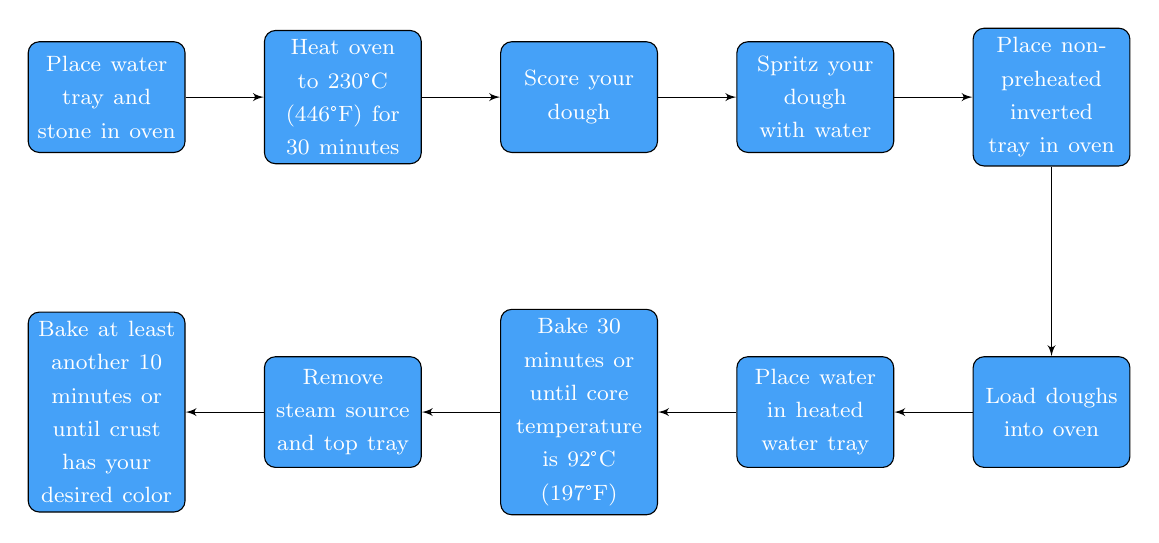
\begin{tikzpicture}[node distance = 3cm, auto]
  \node [block] (init) {\footnotesize Place water tray and stone in oven};
  \node [block, right of=init] (heat_oven) {\footnotesize Heat oven to 230°C (446°F) for 30 minutes};
  \node [block, right of=heat_oven] (score_your_dough) {\footnotesize Score your dough};
  \node [block, right of=score_your_dough] (spritz) {\footnotesize Spritz your dough with water};
  \node [block, right of=spritz] (load_tray) {\footnotesize Place non-preheated inverted tray in oven};
  \node [block, below of=load_tray, node distance=4cm] (load_doughs) {\footnotesize Load doughs into oven};
  \node [block, left of=load_doughs, node distance=3cm] (load_water) {\footnotesize Place water in heated water tray};
  \node [block, left of=load_water, node distance=3cm] (bake) {\footnotesize Bake 30 minutes or until core temperature is 92°C (197°F)};
  \node [block, left of=bake, node distance=3cm] (remove_steam) {\footnotesize Remove steam source and top tray};
  \node [block, left of=remove_steam, node distance=3cm] (finish) {\footnotesize Bake at least another 10 minutes or until crust has your desired color};
  \path [line] (init) -- (heat_oven);
  \path [line] (heat_oven) -- (score_your_dough);
  \path [line] (score_your_dough) -- (spritz);
  \path [line] (spritz) -- (load_tray);
  \path [line] (load_tray) -- (load_doughs);
  \path [line] (load_doughs) -- (load_water);
  \path [line] (load_water) -- (bake);
  \path [line] (bake) -- (remove_steam);
  \path [line] (remove_steam) -- (finish);
\end{tikzpicture}
\end{document}
